%----------------------------------------------------------------------------------------
%	TITLE OF THE HOMEWORK	
%----------------------------------------------------------------------------------------
{\setlength{\parindent}{0pt}
\title{file title} % Article title
\fancyhead[C]{}
\begin{minipage}{0.295\textwidth} % Left side of title section
\raggedright
Tight Binding schemes\\ % Your lecture or course
\footnotesize % Authors text size
%\hfill\\ % Uncomment if right minipage has more lines
Victoria Castor Villegas % Your name, your matriculation number
\medskip\hrule
\end{minipage}
\begin{minipage}{0.4\textwidth} % Center of title section
\centering 
\large % Title text size
diMethylenePyrene cation\\ % Assignment title and number
\normalsize % Subtitle text size
the effect of temperature\\ % Assignment subtitle
\end{minipage}
\begin{minipage}{0.295\textwidth} % Right side of title section
\raggedleft
2022-01-03\\ % Date
\footnotesize % Email text size
%\hfill\\ % Uncomment if left minipage has more lines
victoria.castor@estudiante.uam.es % Your email
\medskip\hrule
\end{minipage}
}
%----------------------------------------------------------------------------------------
%	HOMEWORK CONTENTS
%----------------------------------------------------------------------------------------

\section{\textbf{Computational Details}}

In this work we saw output files given to us, first of all is easy to know that
the main computational program used for the propouse of the study
was the program deMon-Nano \cite{deMonNano} which is a software package for
Density Functional Theory based Tight Binding (DFTTB) calculations. It is part of the
deMon (density of Montréal) program suite \cite{deMon}. Those codes are avaible on
the web pages: \href{http://demon-nano.ups-tlse.fr}{deMonNano} and
\href{http://www.demon-software.com/public_html/program.html#citations}{deMon2k}.

\begin{wrapfigure}{l}{0.42\textwidth}
    \centering
    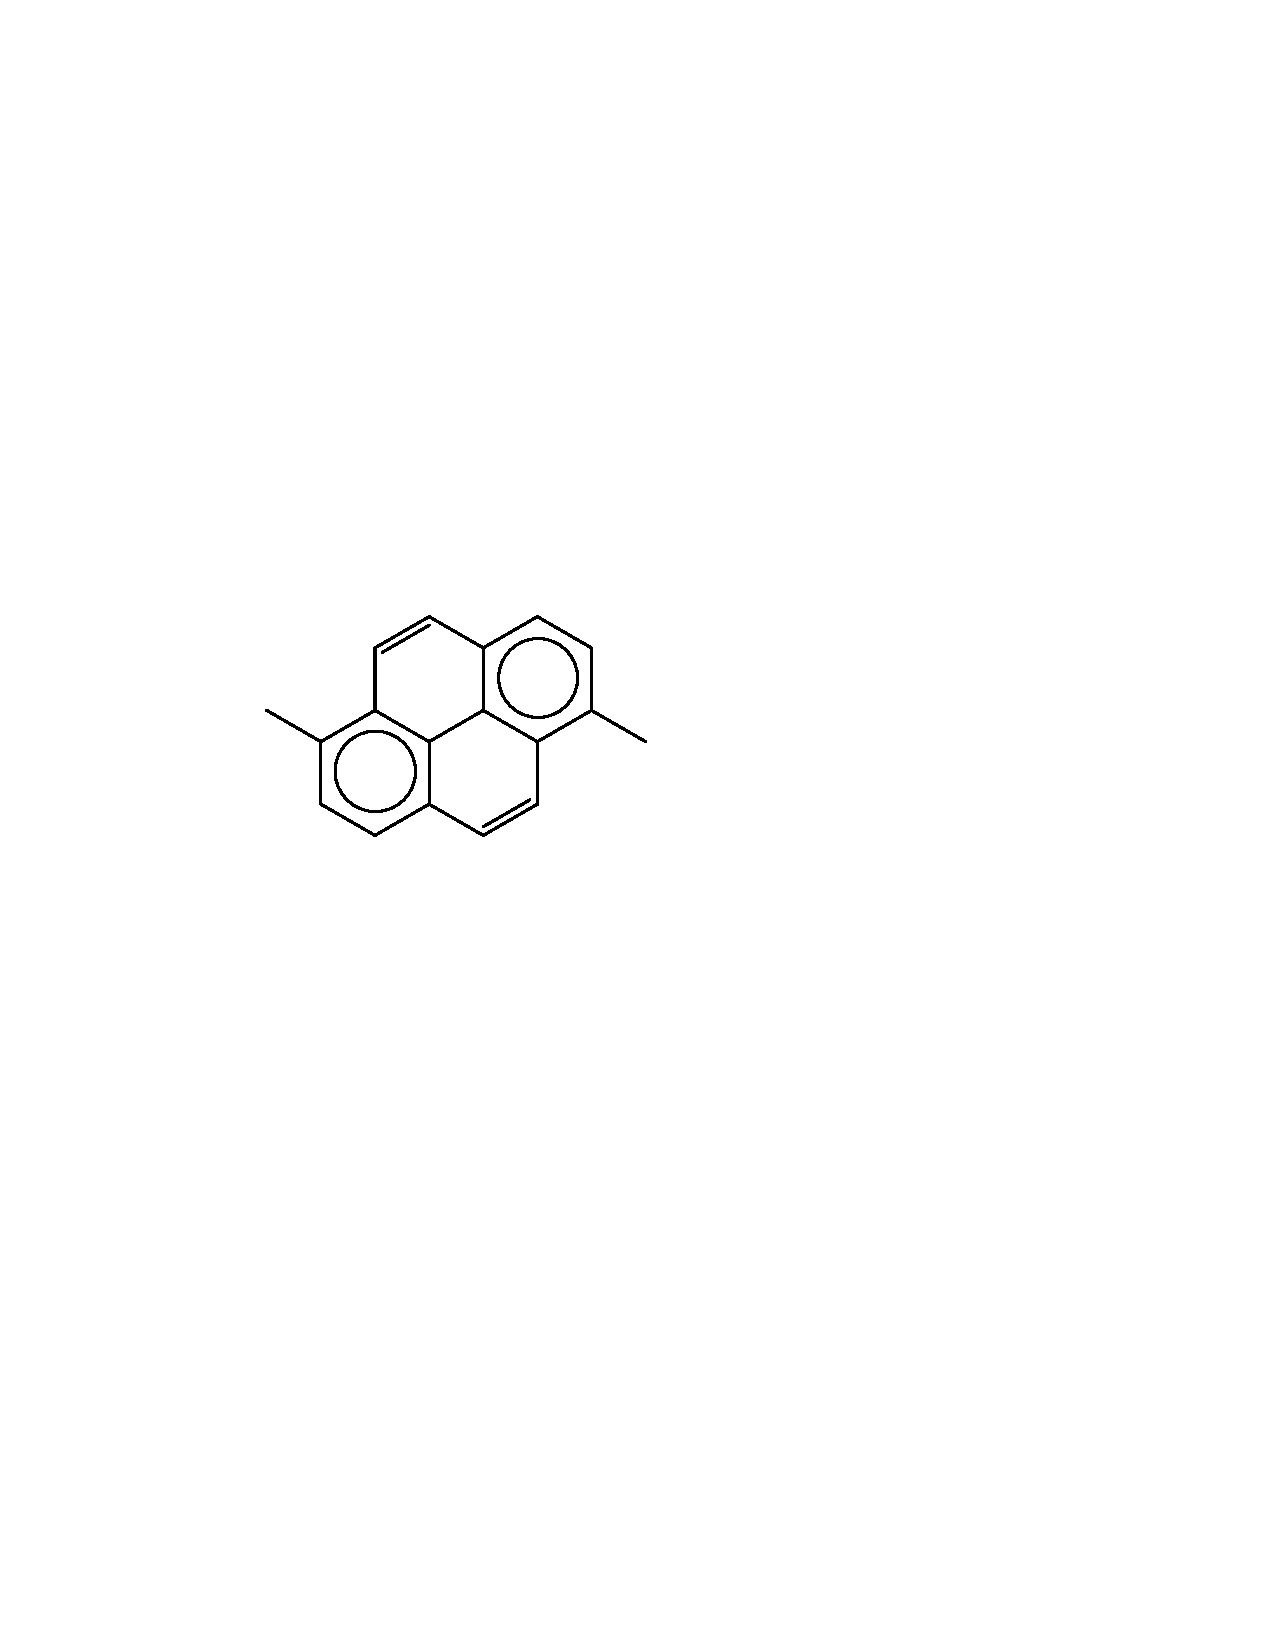
\includegraphics[width=0.42\textwidth]{./img/dimetil}
    \caption{Dimethylenepyrene molecule.}
\label{dimethylenepyrene}
\end{wrapfigure}

Since the output files write down how many time was required for the
calculation we can presume that the number of processadors was four, its
becuase the \texttt{TOTAL TIME} is four times the \texttt{REAL TIME}, the
processadors used. About the memory, the maximum distinated to allocate is
8000.000 MBYTES and DFTB requieres 0.580 MBYTES of allocatable memory.

The starting guess point geometry to optimize was problably taken from
literature or was done with help of some visual representation builder as
Avogadro~\cite{Hanwell2012} or {\sc{GaussView}}~\cite{g16}. In this report we use
{\sc{GnuPlot}}~\cite{gnuplot} for visual representations of plots.

$\,$

\section{\textbf{Step 1}}

Firstly is necessary optimize the molecule geometry at the theory
level that was used. For that propuse on the input file
the next keywords was used:

\begin{itemize}
\item \texttt{DFTB}: theory level is Density Functional based Tight Binding. And \texttt{SCC} to
self-consistent charge variant of DFTB.

\item \texttt{OPTIMIZATION MAX=500}: set the Maximum number of SCC cycles. That just to
expand the default maximum, which is 100.
\end{itemize}

Few words about DFTB, the main point starts taking the density as a sum of some
reference density, adding a small fluctuation: $\rho (\mathbf{r}) =
\rho_0(\mathbf{r}) + \delta\rho (\mathbf{r})$, and expanding the energy (as a
function of $\rho$) into a Taylor series up to a given order.

$$
E[\rho_0 + \delta\rho ] = E_0[\rho_0] + E_1[\rho_0, \delta\rho] + E_2[\rho, (\delta\rho)^2] +
E_3[\rho_0, (\delta\rho)^3] + ...
$$

Consecuently, consider only terms with up to the second order of density fluctuations, the
energy can be expressed as:

\begin{equation}
\begin{split}
E = \sum_{i=1}^N n_i \expval{\hat{H_0}}{\phi_i}
&-\frac12\int\int\frac{\rho_0(\mathbf{r})\rho_0(\mathbf{r'})}{|\mathbf{r}-\mathbf{r'}|}
\dd \mathbf{r}\dd \mathbf{r'}
+E_{\mathrm{xc}[\rho_0]}
-\int\rho_0(\mathbf{r})V_{\mathrm{xc}}[\rho_0(\mathbf{r})]\dd\mathbf{r}
+E_{\mathrm{nn}}+ ...\\\nonumber
&+\frac12\int\int\biggl(\frac1{|\mathbf{r}-\mathbf{r'}|}+\pdv{E_{\mathrm{xc}}}{\rho}{\rho'}\biggr |_{\rho=\rho_0} \biggr)
\delta\rho(\mathbf{r})\delta\rho(\mathbf{r'})\dd\mathbf{r}\dd\mathbf{r'}\nonumber
\end{split}
\end{equation}

The geometry is written down on the same input file, it was not consider any extra
charge for the molecule, \textit{i. e.}, \texttt{CHARGE 0}. The basis are in
\texttt{\textasciitilde /basis/} at the computer where the calculations was carried out, where
was gotten \texttt{\textasciitilde /basis/skf/bio-scc/cc.spl},
\texttt{\textasciitilde /basis/skf/bio-scc/ch.spl}, \newline \texttt{\textasciitilde /basis/skf/bio-scc/hc.spl} and
\texttt{\textasciitilde /basis/skf/bio-scc/hh.spl}

With that input file, the output file was gotten after 12.747 $\mathrm{s}$ of
computing. Really fast, we know that DFTB is roughly three orders of magnitude
faster than DFT which is alredy faster than wavefunction methods.

\section{\textbf{Step 2}}

With the previous calculation, the geometry optimized was taken to compute the
next step,  with the next keyword at the input file \texttt{LRESP} to perform a TDDFTB
calculation Linear Response.

Where the Linear Response TD-DFT(B) only takes into account components of a desntity
fluctuation $\delta\rho (\mathbf{r}, \omega)$ that depend linearly on the
external perturbation, \textit{i.e.}:

$$
\delta\rho (\mathbf{r},\omega) =\int\chi (\mathbf{r},\mathbf{r'},\omega )
\delta V_{ext}(\mathbf{r'}, \omega) \mathrm{d\mathbf{r'}}
$$
\noindent with:
$$
\chi (\mathbf{r},\mathbf{r'},\omega ) = \lim_{\eta \to 0^+} \sum_{k=1}^N \sum_{l=1}^N
(f_k - f_l)\frac{\phi_l(\mathbf{r})\phi_k(\mathbf{r}) \phi_l(\mathbf{r'})\phi_k(\mathbf{r'})}
{\omega - (\varepsilon_l - \varepsilon_k) + i\eta}
$$
\noindent and,
$\delta V_{ext}(\mathbf{r'}, \omega)$ is the linearized time-dependent KS potential,
from:
$$
\hat{V}_{eff}[\rho (\mathbf{r})] = \hat{V}_{\mathrm{ne}}(\mathbf{r}) +
\int\frac{\rho(\mathbf{r'})}{|\mathbf{r-r'}|} \mathrm{d} \mathbf{r'} + 
\hat{V}_{XC}[\rho (\mathbf{r})]
$$

At this point is possible sumarize the next, reading the output file of
these step:

\begin{table}[h]
\caption{Summary Table of Energy, $E\mathrm{_h}$ unit}
\begin{tcolorbox}[tab2,tabularx={X||Y},title=Summary Table,boxrule=0.5pt]
Description		& Energy \\\hline\hline
DFTB Electronic		& -36.64694927 \\\hline
DFTB Band		& -36.65447764 \\\hline
DFTB Repulsive		& 1.16712873   \\\hline
DFTB Coulomb		& 0.00752837   \\\hline
DFTB Total		& -35.47982055 \\\hline
DFTB HOMO-LUMO gap 	& 0.0553812 \\\hline
DFTB (HOMO)-(HOMO-1) gap & 0.0431804 \\
\end{tcolorbox}
\label{distance}
\end{table}

Also, at this step we can know about the spectrum, particularly about the transitions. About
its energy, oscillation strength, that for singlets and triplets, as we shown in the Table
\ref{singulete_triplete}. Where we can see the allowed excitations (Osz. strength different
than zero).

\newpage

% Table generated by Excel2LaTeX from sheet 'Sheet1'
\begin{table}[htbp]
  \centering
  \caption{Transitions for diMethylenePyrene}
    \begin{tabular}{rrlrrl}
    \multicolumn{1}{l}{w [eV]} & \multicolumn{1}{l}{Osz. strength} & Transition & \multicolumn{1}{l}{Weight} & \multicolumn{1}{l}{E\_sp [eV]} & Sym. \\
    2.389 & 0.3985879 & 42 -> 43 & 0.602 & 1.507 & S \\
    2.771 & 0.0000000 & 41 -> 43 & 0.691 & 2.682 & S \\
    3.188 & 0.0000000 & 39 -> 43 & 0.568 & 3.141 & S \\
    3.225 & 0.0173636 & 40 -> 43 & 0.796 & 3.083 & S \\
    3.483 & 0.0000000 & 42 -> 46 & 0.428 & 3.657 & S \\
    3.717 & 0.0000000 & 38 -> 43 & 1.000 & 3.717 & S \\
    3.849 & 0.0402239 & 42 -> 45 & 0.645 & 3.563 & S \\
    3.917 & 0.0089270 & 37 -> 43 & 0.761 & 3.802 & S \\
    3.933 & 0.0000000 & 36 -> 43 & 1.000 & 3.933 & S \\
    4.264 & 0.0000000 & 42 -> 46 & 0.455 & 3.657 & S \\
    1.319 & 0.0000000 & 42 -> 43 & 1.139 & 1.507 & T \\
    2.542 & 0.0000000 & 41 -> 43 & 0.918 & 2.682 & T \\
    2.849 & 0.0000000 & 42 -> 44 & 0.855 & 2.918 & T \\
    3.01  & 0.0000000 & 39 -> 43 & 0.958 & 3.141 & T \\
    3.047 & 0.0000000 & 40 -> 43 & 1.006 & 3.083 & T \\
    3.528 & 0.0000000 & 42 -> 45 & 1.001 & 3.563 & T \\
    3.573 & 0.0000000 & 42 -> 46 & 0.981 & 3.657 & T \\
    3.689 & 0.0000000 & 37 -> 43 & 0.957 & 3.802 & T \\
    3.717 & 0.0000000 & 38 -> 43 & 1.000 & 3.717 & T \\
    3.933 & 0.0000000 & 36 -> 43 & 1.000 & 3.933 & T \\
    \end{tabular}%
  \label{singulete_triplete}%
\end{table}%




\section{\textbf{Step 3}}

Now, with the information obtainied by the other two steps, was posible to start
a compute for the spectrum, with four particular sub-steps, that four substeps changing the
next keyword \texttt{MDYNAMICS RANDOM=} with the values 200, 500, 1000 and
1500.

The first keyword \texttt{MDYNAMICS} activates the Born-Oppenheimer molecular
dynamic, and the second one \texttt{RANDOM=} starts a trajectory using random
initial velocites, which have no net momentum or angular momentum and give the
requested temperature specified after the equal sign.

That means, that the next subteps will provide the spectra with
200 K, 500 K, 1000 K and 1500 K.
Even if the molecule are not physical chemistry avialbe at that temperature, we
are not in that analysis.

Finally, the last keyword \texttt{TIMESTEP} specifies the time step of the molecular dynamic
in femtosecond, for all four cases the \texttt{TIMESTEP} was 0.5.

In all cases we have a detailed output for spectra and another one with just
the main points to the spectra plots. We are ploting the
\texttt{spectrum\_final.out} for the 4 substeps in the Figure \ref{substeps}.
Spectrums that we will analize.

Is possible to see the more themperature the more interference. Not having resolution
with 5000 K or more, and being not readable with 1000 K, where would be impossible to
know which molecule we would have (even with experimental data).

Looking at the spectra with the lowest temperature and since we know the
molecule (diMethylenePyrene cation) we can elucidate how the signals are in. 
For the H atoms at the methyl the spectra has a signal that integrate 4. We guess that is
the signal arround 2 ppm.

Another signal would appear because the two H atoms at 2
and 7 molecule possition. That signal would appear close to 3 ppm. Finally the
$\mathrm{H^1}$-NMR would have had a signal for all the others H atoms,
inegrating for 6 with a really closer signals for all of these H atoms, since
theirs chemical shift are basically the same arround 4 ppm.

That correspond, more or less with what we see. Knowing now that we sorted out the H
atoms in three ways. All four sprectra ``has'' that. However, just at 200
and maybe at 500 K is possible to elucidate the integral values, but not
the best.

Experementally we know that the $\mathrm{H^1}$-NMR are done with temperatures
upper, but closer to liquid $\mathrm{N}_2$, $80 \mathrm{K}$. Now we know, with 200 K we
are at approximation that spend really few computing time.

\begin{figure}[h]
\centering
\begin{subfigure}[b]{0.48\linewidth}
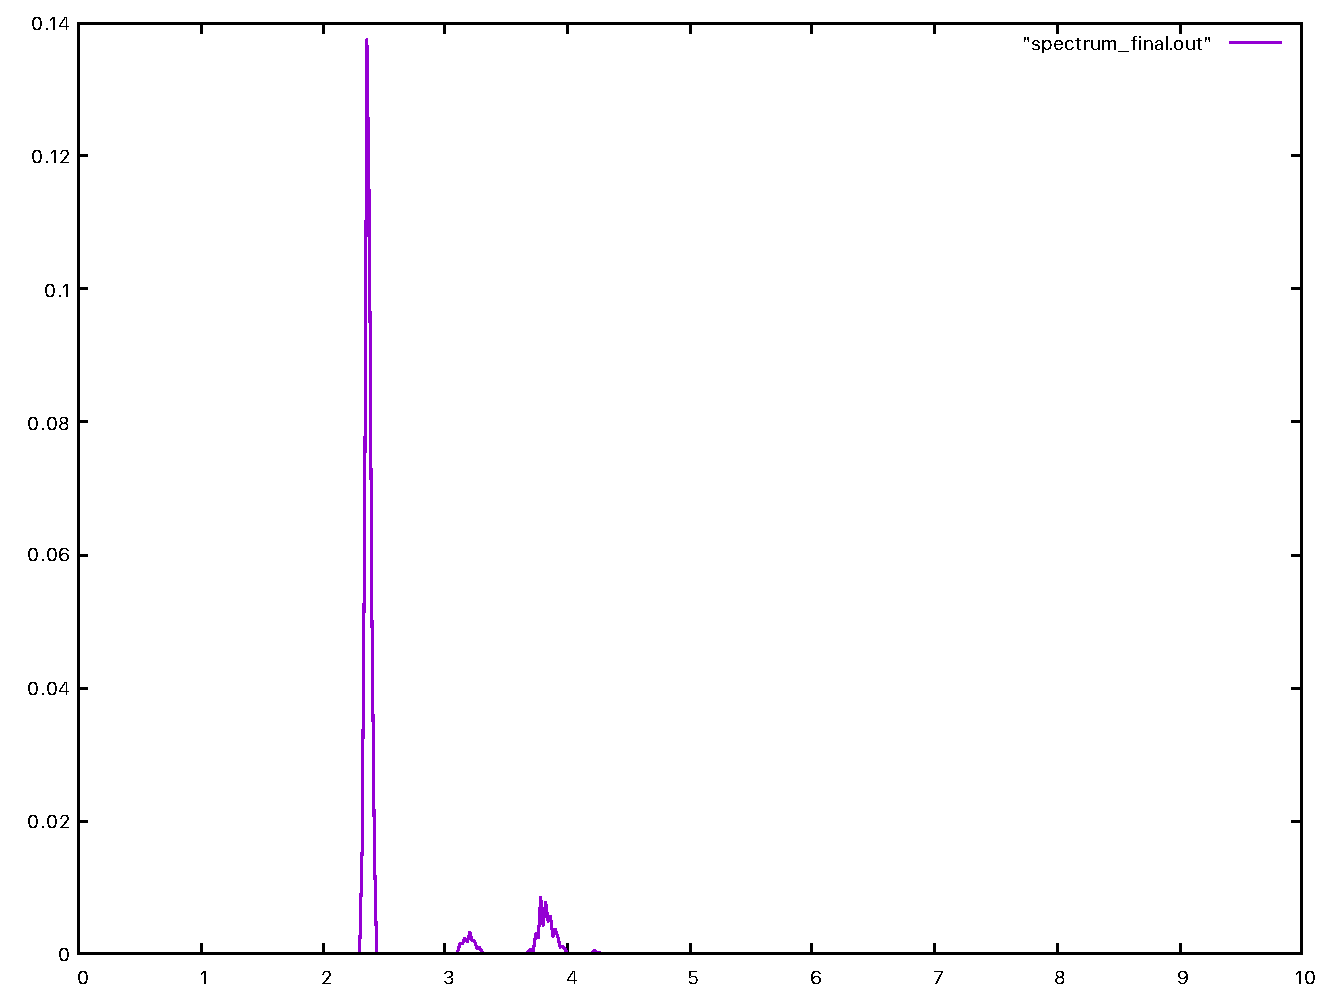
\includegraphics[width=\linewidth]{./img/spectra_a}
\caption{200 K.}
\end{subfigure}
\begin{subfigure}[b]{0.48\linewidth}
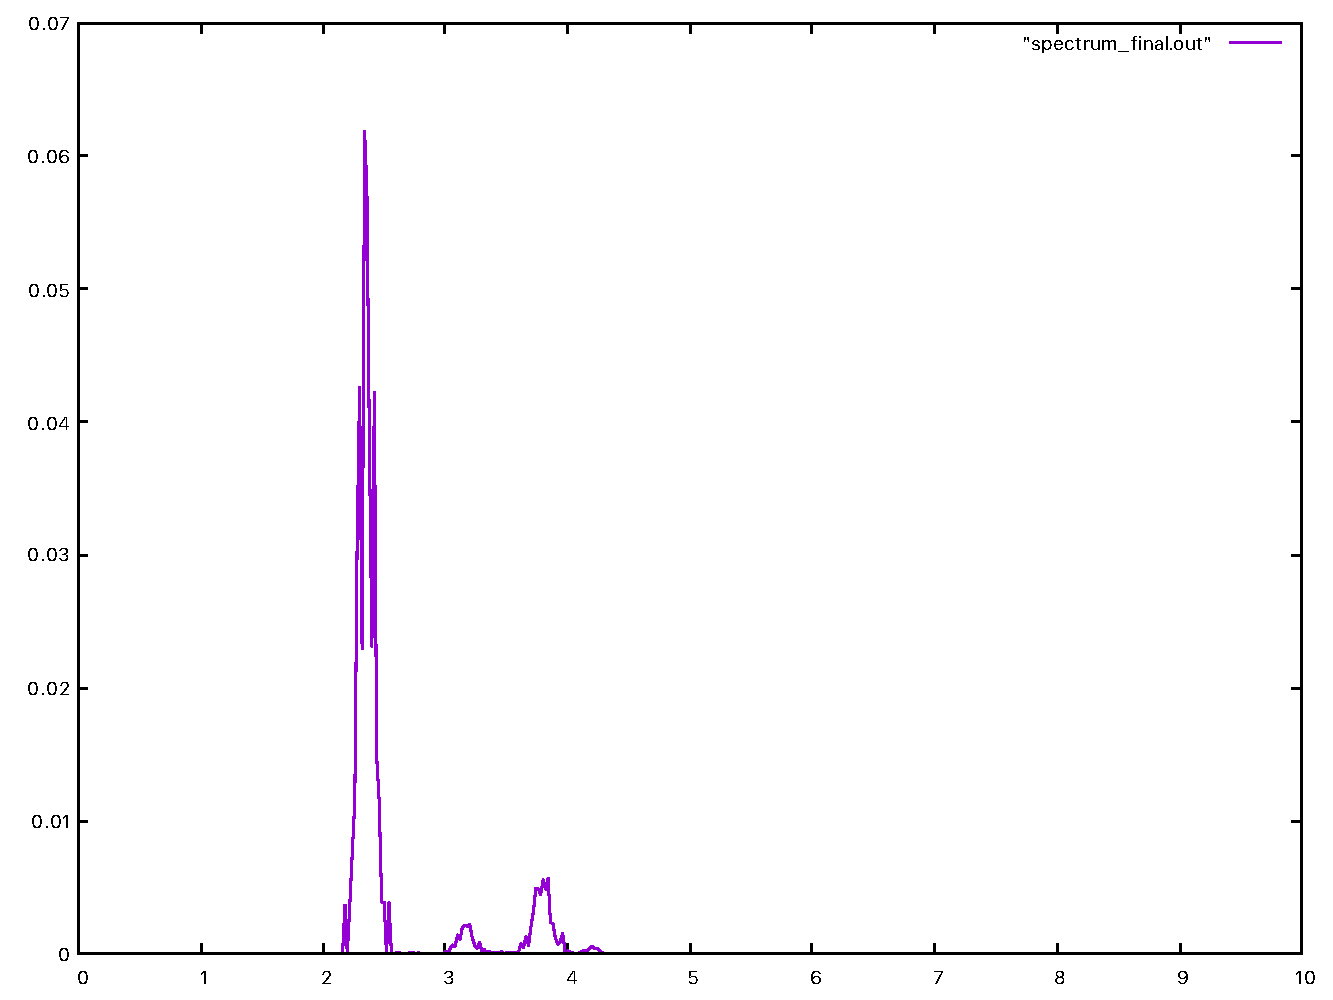
\includegraphics[width=\linewidth]{./img/spectra_b}
\caption{500 K.}
\end{subfigure}
\begin{subfigure}[b]{0.48\linewidth}
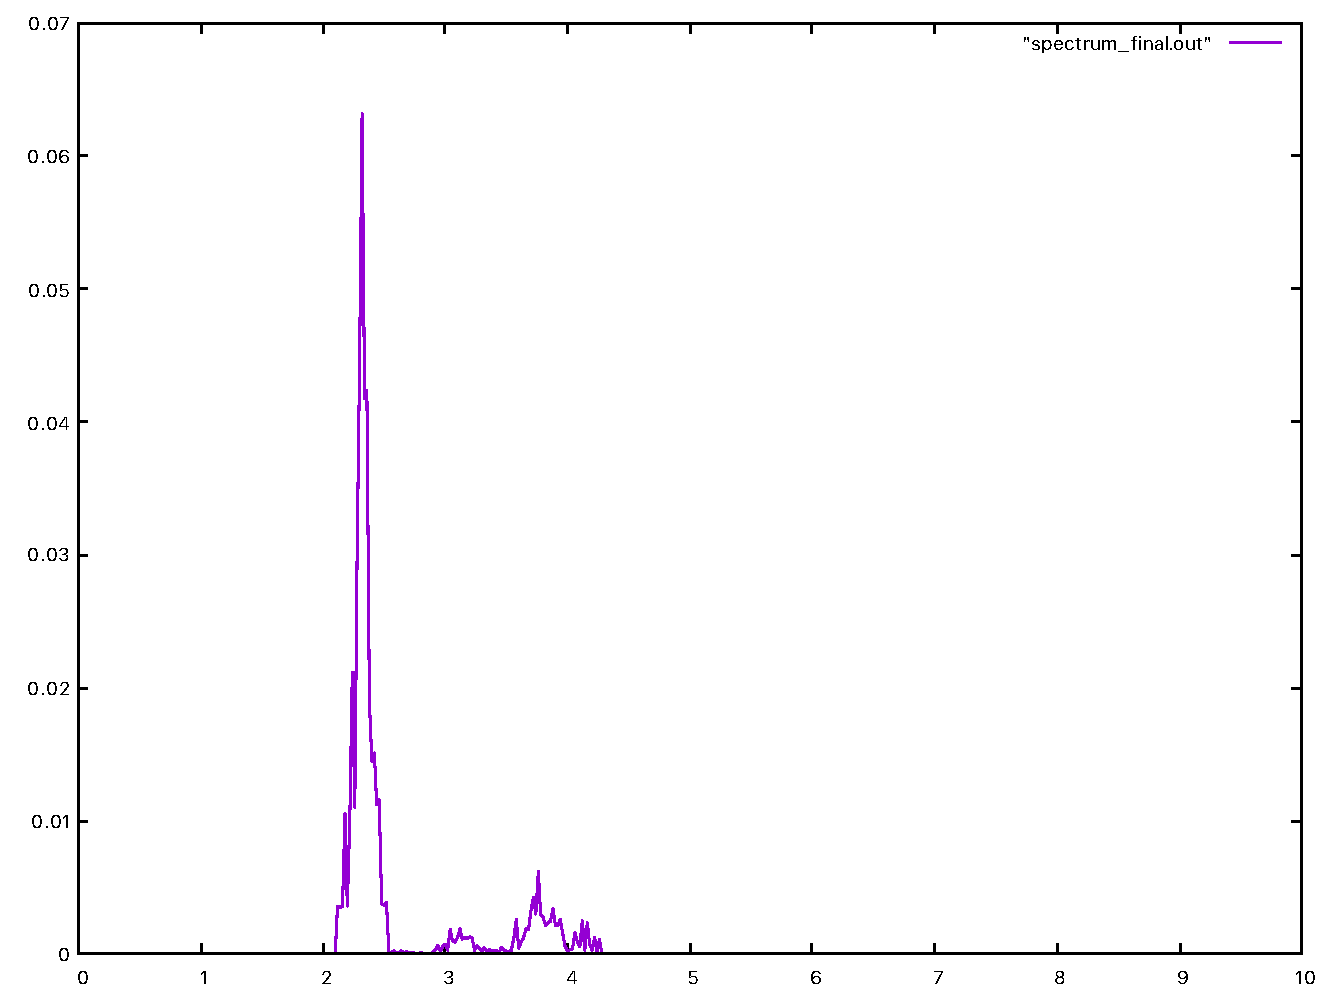
\includegraphics[width=\linewidth]{./img/spectra_c}
\caption{1000 K.}
\end{subfigure}
\begin{subfigure}[b]{0.48\linewidth}
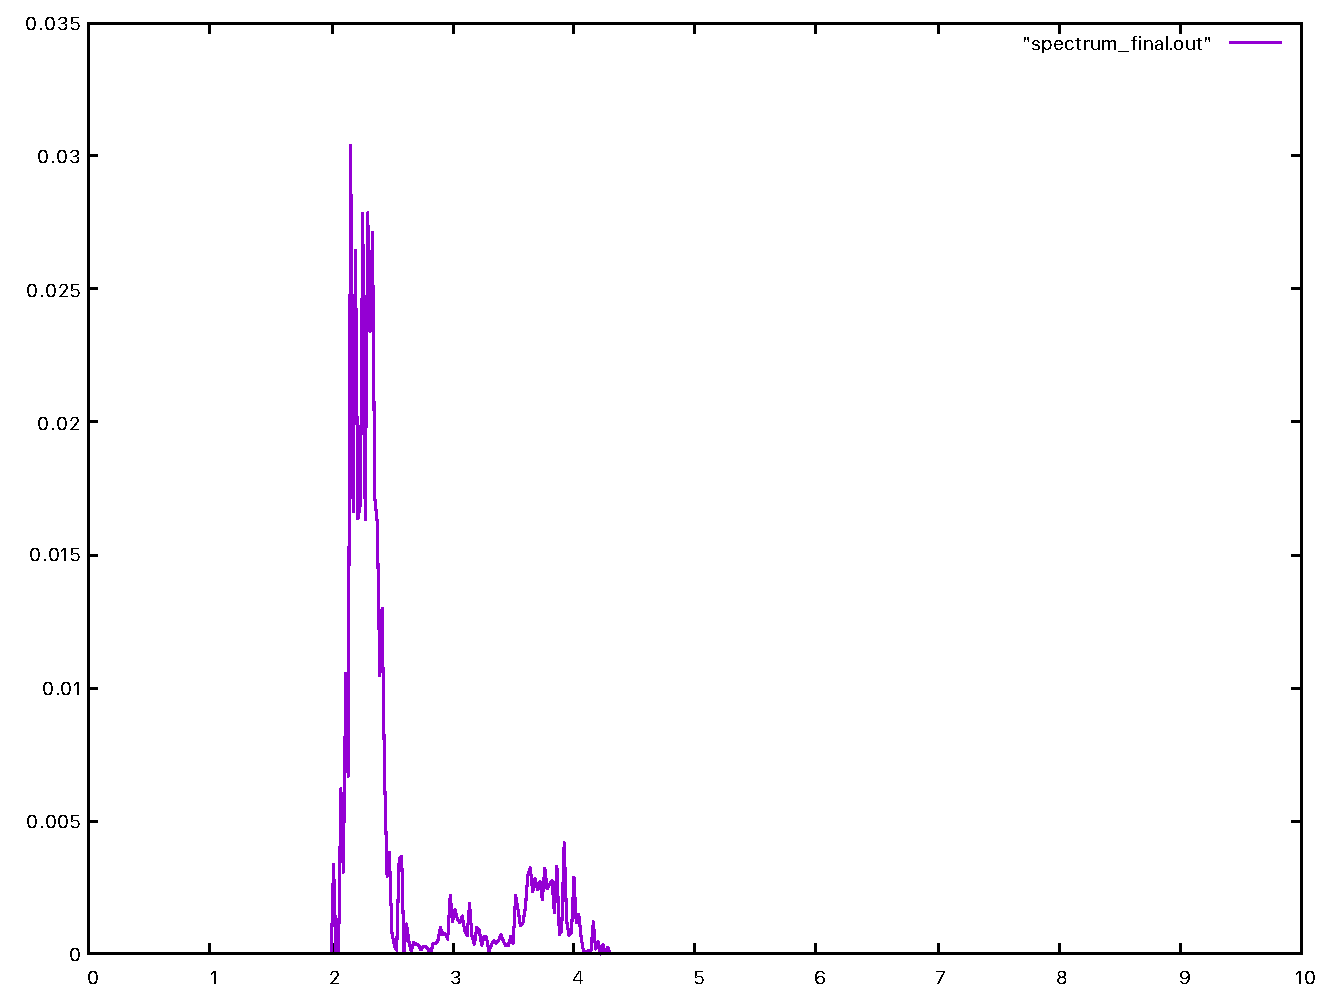
\includegraphics[width=\linewidth]{./img/spectra_d}
\caption{1500 K.}
\end{subfigure}
\caption{Substeps a, b, c \& d}
\label{substeps}
\end{figure}



